\documentclass[11pt,a4paper]{article}

% ---------------------------------------------------------------------------
% Packages
% ---------------------------------------------------------------------------
\usepackage[T1]{fontenc}
\usepackage[utf8]{inputenc}
\usepackage{lmodern}
\usepackage{mathptmx}
\usepackage[margin=2.3cm]{geometry}
\usepackage{microtype}
\usepackage{amsmath,amssymb,amsthm}
\usepackage{bm}
\usepackage{booktabs}
\usepackage{multirow}
\usepackage{array}
\usepackage{graphicx}
\usepackage[font=small,labelfont=bf,skip=5pt]{caption}
\usepackage{subcaption}
\usepackage{xcolor}
\usepackage{tikz}
\usetikzlibrary{arrows.meta,positioning,calc,decorations.pathreplacing,fit}
\usepackage{algorithm}
\usepackage{algpseudocode}
\usepackage{listings}
\usepackage{enumitem}
\usepackage{placeins}
\usepackage[numbers,sort&compress]{natbib}
\usepackage[colorlinks=true,linkcolor=cglink,citecolor=cglink,urlcolor=cglink]{hyperref}
\usepackage[capitalise,noabbrev]{cleveref}

\definecolor{cglink}{HTML}{1F4E79}
\definecolor{cgblue}{HTML}{2A78D6}
\definecolor{cgorange}{HTML}{EB6834}
\definecolor{cggray}{HTML}{8A8984}
\definecolor{cgpale}{HTML}{F2F5F9}

\setlist{nosep,leftmargin=1.4em}
% Let figures and tables share pages with text instead of forming sparse float pages.
\renewcommand{\topfraction}{0.9}
\renewcommand{\bottomfraction}{0.8}
\renewcommand{\textfraction}{0.07}
\renewcommand{\floatpagefraction}{0.8}
\setcounter{topnumber}{3}
\setcounter{bottomnumber}{2}
\setcounter{totalnumber}{5}
\setlength{\parskip}{0.35em}
\renewcommand{\arraystretch}{1.12}

\newtheorem{proposition}{Proposition}
\newtheorem{definition}{Definition}
\theoremstyle{remark}
\newtheorem*{remark}{Remark}

\lstdefinestyle{py}{
  language=Python, basicstyle=\ttfamily\footnotesize, keywordstyle=\color{cglink}\bfseries,
  commentstyle=\color{cggray}\itshape, stringstyle=\color{cgorange!80!black},
  backgroundcolor=\color{cgpale}, frame=single, rulecolor=\color{cggray!40},
  framesep=4pt, xleftmargin=6pt, xrightmargin=6pt, showstringspaces=false,
  breaklines=true, columns=fullflexible, keepspaces=true, aboveskip=6pt, belowskip=6pt}

% Every number quoted in the prose is generated from the result files.
% Auto-generated by make_paper_assets.py -- do not edit by hand.
\newcommand{\bestLeakDeadPct}{96}
\newcommand{\bestLeakLambda}{10}
\newcommand{\bestLeakMode}{mean}
\newcommand{\bestLeakRouting}{0.0003}
\newcommand{\bestLeakValue}{0.0020}
\newcommand{\bestRoutAlivePct}{83}
\newcommand{\bestRoutLeak}{0.296}
\newcommand{\bestRoutValue}{0.40}
\newcommand{\blockOffPositive}{4}
\newcommand{\blockPositive}{19}
\newcommand{\blockRuns}{5}
\newcommand{\blockSig}{10}
\newcommand{\blockSigHolm}{1}
\newcommand{\blockSigTauFifty}{1}
\newcommand{\blockSigTauFive}{3}
\newcommand{\blockSigTauTen}{4}
\newcommand{\blockSigTauTwenty}{2}
\newcommand{\blockSignP}{2.0\times10^{-5}}
\newcommand{\blockTotal}{20}
\newcommand{\budget}{10}
\newcommand{\cgGptSent}{+0.109}
\newcommand{\cgGptTox}{+0.133}
\newcommand{\cgPGptSent}{$<$0.001}
\newcommand{\cgPGptTox}{0.879}
\newcommand{\cgPQwenSent}{0.004}
\newcommand{\cgPQwenTox}{0.007}
\newcommand{\cgQwenSent}{+0.277}
\newcommand{\cgQwenTox}{+0.127}
\newcommand{\contrastFVUlamOne}{0.250}
\newcommand{\contrastFVUlamTen}{1.03}
\newcommand{\contrastRoutLamOne}{0.36}
\newcommand{\degenCorrMax}{-0.28}
\newcommand{\dimGptSent}{+0.404}
\newcommand{\dimGptTox}{+0.130}
\newcommand{\dimQwenSent}{+0.413}
\newcommand{\dimQwenTox}{+0.044}
\newcommand{\dimSentSAEbetter}{0}
\newcommand{\dimSentSAEworse}{12}
\newcommand{\dimSentTotal}{12}
\newcommand{\dimToxSAEbetter}{3}
\newcommand{\dimToxSAEworse}{0}
\newcommand{\dimToxTotal}{8}
\newcommand{\dissBUnw}{-0.447}
\newcommand{\dissBWan}{+0.184}
\newcommand{\dissGUnw}{+0.183}
\newcommand{\dissGWan}{-0.411}
\newcommand{\dissRUnw}{-0.039}
\newcommand{\dissRWan}{+0.001}
\newcommand{\evVanGPT}{80}
\newcommand{\evVanQwen}{96}
\newcommand{\fvuCGGPT}{0.277}
\newcommand{\fvuCGQwen}{0.066}
\newcommand{\fvuVanGPT}{0.203}
\newcommand{\fvuVanQwen}{0.045}
\newcommand{\layerDisagree}{4}
\newcommand{\layerFracMax}{85}
\newcommand{\layerFracMin}{27}
\newcommand{\layerGptAUC}{0.816}
\newcommand{\layerGptLoss}{45}
\newcommand{\layerGptProbe}{11}
\newcommand{\layerGptSteer}{7}
\newcommand{\layerScans}{4}
\newcommand{\leakRatioBestVsRout}{146}
\newcommand{\leakRoutingCorr}{+0.03}
\newcommand{\nPrimaryRuns}{5}
\newcommand{\nRuns}{6}
\newcommand{\nSynthSeeds}{20}
\newcommand{\penformConfigs}{12}
\newcommand{\penformSeeds}{2}
\newcommand{\qtoxLfifteenEff}{+0.062}
\newcommand{\qtoxLfifteenPPL}{37.6}
\newcommand{\qtoxLtenEff}{+0.056}
\newcommand{\qtoxLtenPPL}{6.5}
\newcommand{\scarGptSent}{+0.118}
\newcommand{\scarGptTox}{+0.194}
\newcommand{\scarPGptSent}{$<$0.001}
\newcommand{\scarPGptTox}{0.022}
\newcommand{\scarPQwenSent}{$<$0.001}
\newcommand{\scarPQwenTox}{0.075}
\newcommand{\scarQwenSent}{+0.147}
\newcommand{\scarQwenTox}{+0.075}
\newcommand{\specMax}{16.6}
\newcommand{\specMaxBuf}{4.33}
\newcommand{\specMaxLamFive}{14.0}
\newcommand{\specNoBufLamFive}{0.91}
\newcommand{\specNoBufLamOne}{1.5}
\newcommand{\specOffMax}{1.65}
\newcommand{\specOffMin}{0.99}
\newcommand{\sqFVUspread}{1.2\times10^{-4}}
\newcommand{\sqLeakLamThirty}{0.435}
\newcommand{\sqLeakLamZero}{0.495}
\newcommand{\sqPenShare}{0.5}
\newcommand{\sqPenTermThirty}{8.7\times10^{-4}}
\newcommand{\sqRoutMax}{0.012}
\newcommand{\synthBAliveMin}{100}
\newcommand{\synthRouting}{0.35}
\newcommand{\synthRoutingOff}{0.010}
\newcommand{\vanFVUpenform}{0.173}
\newcommand{\vsSSVgptPmax}{0.40}
\newcommand{\vsSSVgptPmin}{0.24}
\newcommand{\vsSSVgptPositive}{3}
\newcommand{\vsSSVgptSig}{0}
\newcommand{\vsSSVgptTotal}{4}
\newcommand{\vsSSVqwenPositive}{8}
\newcommand{\vsSSVqwenPrimSig}{4}
\newcommand{\vsSSVqwenPrimTotal}{6}
\newcommand{\vsSSVqwenSig}{6}
\newcommand{\vsSSVqwenSigHolm}{3}
\newcommand{\vsSSVqwenTotal}{8}
\newcommand{\vsScarQwenSig}{1}
\newcommand{\vsScarSig}{1}
\newcommand{\vsScarTotal}{12}


% Notation
\newcommand{\R}{\mathbb{R}}
\newcommand{\E}{\mathbb{E}}
\newcommand{\z}{\mathbf{z}}
\newcommand{\x}{\mathbf{x}}
\newcommand{\h}{\mathbf{h}}
\newcommand{\Gset}{\mathcal{G}}
\newcommand{\Bset}{\mathcal{B}}
\newcommand{\Nset}{\mathcal{N}}
\newcommand{\ntag}{n_{\mathrm{tag}}}
\newcommand{\dec}{\operatorname{dec}}
\newcommand{\enc}{\operatorname{enc}}
\newcommand{\TopK}{\operatorname{TopK}}
\newcommand{\ReLU}{\operatorname{ReLU}}
\newcommand{\FVU}{\operatorname{FVU}}

\title{\vspace{-1.2em}\textbf{Where Should a Concept Live?\\[2pt]
\large Latent Capacity Allocation and the Role of a Neutral Buffer\\ in Supervised Sparse Autoencoders}}
\author{Varanasi Sathveek \qquad Vanamala Aravind \qquad Pula Naga Manikanta \qquad K.\ Hima Bindu\\[4pt]
\normalsize Department of Computer Science \& Engineering\\
\normalsize National Institute of Technology Andhra Pradesh, India}
\date{}

\begin{document}
\maketitle

% ===========================================================================
\begin{abstract}
\noindent
Sparse autoencoders (SAEs) decompose language-model activations into interpretable
features, and recent supervised variants place a target concept at a known position in the
latent space, either by conditioning a single latent during training or by selecting latents
after training. Neither asks how much latent \emph{capacity} a concept should receive, nor
where features shared between two opposing classes should live. We study
\emph{Class-Grouped Sparse Autoencoders} (CG-SAE), which partition the latent space before
training into a wanted block, an unwanted block and an unpenalised \emph{neutral buffer}, so
that an unwanted behaviour can later be removed by address rather than by search. We first
show that the natural cross-group penalty fails under realistic sparsity in two distinct ways:
a squared-mean penalty is numerically inert, and every suppression-only penalty admits a
vacuous minimiser in which both tagged blocks fall silent. We replace it with a contrastive
routing objective and show that the leakage metric used to evaluate such partitions is
uninformative about whether they work (correlation with routing $r=\leakRoutingCorr$; the
best-scoring configuration has a \bestLeakDeadPct\% dead block). Across GPT-2 and
Qwen2.5-1.5B on sentiment and toxicity, and under a protocol that matches sparsity,
intervention width and fluency cost, ablating the reserved block reduces the target behaviour
more than ablating a size-matched random block in \blockPositive{} of \blockTotal{}
run--configuration cells (sign test $p=\blockSignP$). In a controlled synthetic setting the
buffer is the mechanism: ablation specificity falls from \specMax$\times$ to chance as the
buffer is removed. Under identical post-hoc latent selection, a CG-SAE dictionary steers better
than a vanilla SAE on Qwen2.5-1.5B (\vsSSVqwenSig{} of \vsSSVqwenTotal{} tests) but not on GPT-2
(\vsSSVgptSig{} of \vsSSVgptTotal{}), and against difference-in-means steering the ranking
is task-dependent. Finally, in all \layerScans{} layer scans the layer at which a concept is
most linearly decodable is not the layer at which it is most efficiently steered.
\end{abstract}

\noindent\textbf{Keywords:} mechanistic interpretability; sparse autoencoders; activation
steering; representation engineering; model editing; evaluation methodology

% ===========================================================================
\section{Introduction}
\label{sec:intro}

Controlling a specific behaviour of a language model without disturbing the rest is difficult
because features are stored in superposition: a model represents many more concepts than it
has dimensions, so concept directions overlap and any intervention aimed at one collaterally
moves others~\citep{elhage2022toy}. Sparse autoencoders (SAEs) address this by re-expressing
residual-stream activations in an overcomplete basis under a sparsity constraint, recovering
latents that are closer to single concepts~\citep{bricken2023monosemanticity,cunningham2024sparse,templeton2024scaling,gao2024scaling}.

A standard SAE, however, imposes no semantic organisation on its latents. To steer or remove a
concept one must first \emph{find} the latents that carry it. Supervised variants remove part
of this search. SCAR~\citep{harle2024scar} conditions one latent on a concept label during
training; SAE-SSV~\citep{he2025saessv} learns a supervised subspace from a pretrained SAE;
other work adds probe, graph or contrastive terms to the SAE
objective~\citep{yeon2025gsae,kim2026saeparate}. These methods implicitly take one of two
positions on \emph{capacity}: the concept occupies either a single dimension, or an
unspecified set that is discovered afterwards.

We ask the capacity question directly: \emph{how many latents should a concept receive, and
where should features that are genuinely shared between two opposing classes reside?} We
study Class-Grouped Sparse Autoencoders (CG-SAE), which reserve a contiguous block of
$\ntag=\lfloor\tau m\rfloor$ latents for each of a wanted and an unwanted class, and leave the
remaining latents as an unpenalised \emph{neutral buffer} (\cref{fig:method}). If training
routes the unwanted behaviour into its block, that behaviour can be removed at inference by
zeroing a fixed index range: no probing, no ranking and no labelled data at intervention time.

\paragraph{Contributions.}
\begin{enumerate}
  \item \textbf{A capacity-allocation formulation} of supervised SAEs with an explicit neutral
        buffer whose width $\tau$ is a controllable parameter (\cref{sec:method}).
  \item \textbf{An analysis of cross-group objectives under sparsity.} The squared-mean penalty
        of our preliminary work is numerically inert at realistic sparsity, and every
        suppression-only penalty has a vacuous minimiser in which the tagged blocks are
        silent (\cref{prop:silent}). We propose a contrastive routing objective that excludes
        it (\cref{sec:objectives}).
  \item \textbf{An evaluation methodology.} We show that the leakage metric is uncorrelated with
        whether a partition works, and replace it with routing and occupancy measures; and we
        evaluate interventions at a \emph{matched fluency budget}, with a delta-form
        intervention that charges an edit only for itself (\cref{sec:setup}).
  \item \textbf{Empirical findings} across two models, two concept axes and a 20-seed synthetic
        testbed: the reserved block localises the concept; the buffer is what makes it
        specific; training with the partition improves steering over a vanilla SAE at the
        larger scale only; and the ranking against difference-in-means steering is task-dependent
        (\cref{sec:results}).
  \item \textbf{A layer-selection result}: across four layer scans, the most decodable layer is
        never the most steerable one (\cref{sec:layers}).
\end{enumerate}

\paragraph{Relation to our preliminary study.}
This paper supersedes our earlier CG-SAE report. An audit of that implementation
(\cref{app:audit}) found that its headline steering experiment did not exercise the partition,
that it compared outputs from two different decoding procedures, and that the autoencoder was
dense rather than sparse. All results here come from a rebuilt pipeline designed to close
those gaps, with baselines and null controls the preliminary study lacked.

\begin{figure}[t]
\centering
\resizebox{\linewidth}{!}{%
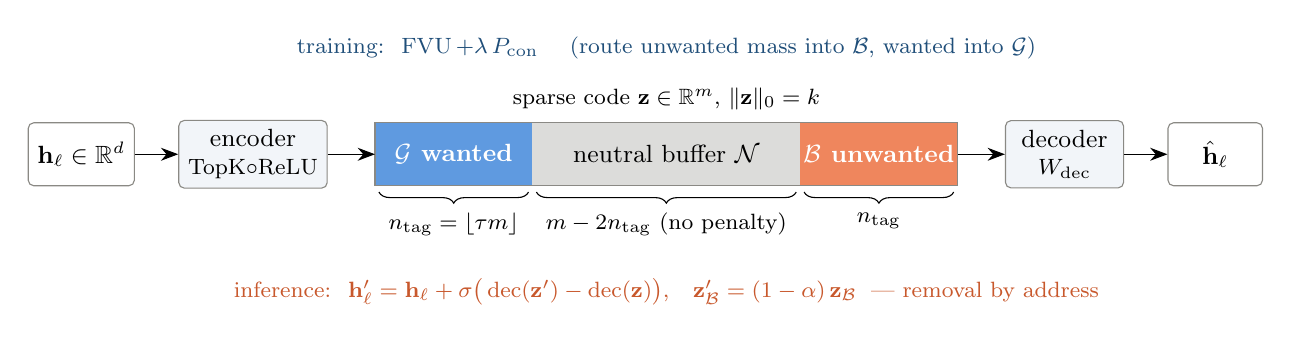
\begin{tikzpicture}[
  font=\small, >={Stealth[length=2.2mm]},
  box/.style={draw=cggray, rounded corners=2pt, minimum height=0.8cm, align=center, fill=white},
  op/.style={draw=cggray, rounded corners=2pt, minimum height=0.8cm, minimum width=1.5cm, align=center, fill=cgpale}]
  \node[box, minimum width=1.3cm] (h) at (0,0) {$\h_\ell\in\R^{d}$};
  \node[op, right=0.55cm of h] (enc) {encoder\\[-1pt]\footnotesize $\TopK\!\circ\!\ReLU$};
  % latent vector: three blocks
  \coordinate (z0) at ($(enc.east)+(0.6,-0.4)$);
  \fill[cgblue!75]   (z0) rectangle ++(2.0,0.8);
  \fill[cggray!30]   ($(z0)+(2.0,0)$) rectangle ++(3.4,0.8);
  \fill[cgorange!80] ($(z0)+(5.4,0)$) rectangle ++(2.0,0.8);
  \draw[cggray] (z0) rectangle ++(7.4,0.8);
  \node[white, font=\small\bfseries] at ($(z0)+(1.0,0.4)$) {$\Gset$ wanted};
  \node[font=\small] at ($(z0)+(3.7,0.4)$) {neutral buffer $\Nset$};
  \node[white, font=\small\bfseries] at ($(z0)+(6.4,0.4)$) {$\Bset$ unwanted};
  \draw[decorate,decoration={brace,amplitude=4pt,mirror}] ($(z0)+(0.05,-0.08)$) -- ++(1.9,0)
     node[midway,below=4pt,font=\footnotesize]{$\ntag=\lfloor\tau m\rfloor$};
  \draw[decorate,decoration={brace,amplitude=4pt,mirror}] ($(z0)+(2.05,-0.08)$) -- ++(3.3,0)
     node[midway,below=4pt,font=\footnotesize]{$m-2\ntag$ (no penalty)};
  \draw[decorate,decoration={brace,amplitude=4pt,mirror}] ($(z0)+(5.45,-0.08)$) -- ++(1.9,0)
     node[midway,below=4pt,font=\footnotesize]{$\ntag$};
  \node[font=\footnotesize, above=1pt] at ($(z0)+(3.7,0.8)$) {sparse code $\z\in\R^{m}$, $\|\z\|_0=k$};
  \node[op, right=0.6cm of {$(z0)+(7.4,0.4)$}] (dec) {decoder\\[-1pt]\footnotesize $W_{\mathrm{dec}}$};
  \node[box, minimum width=1.2cm, right=0.55cm of dec] (hh) {$\hat{\h}_\ell$};
  \draw[->] (h) -- (enc);
  \draw[->] (enc.east) -- ($(z0)+(0,0.4)$);
  \draw[->] ($(z0)+(7.4,0.4)$) -- (dec);
  \draw[->] (dec) -- (hh);
  % training signal
  \node[font=\footnotesize, align=center, text=cglink] (loss) at ($(z0)+(3.7,1.75)$)
     {training: $\;\FVU + \lambda\,P_{\mathrm{con}}$ \quad(route unwanted mass into $\Bset$, wanted into $\Gset$)};
  % intervention
  \node[font=\footnotesize, align=left, text=cgorange!85!black, anchor=north] (int) at ($(z0)+(3.7,-1.05)$)
     {inference: $\;\h'_\ell=\h_\ell+\sigma\big(\dec(\z')-\dec(\z)\big)$,\quad
      $\z'_{\Bset}=(1-\alpha)\,\z_{\Bset}$ \;--- removal by address};
\end{tikzpicture}}
\caption{\textbf{CG-SAE.} The $m$ latents of a TopK SAE are partitioned \emph{before training}
into a wanted block $\Gset$, an unwanted block $\Bset$ and an unpenalised neutral buffer
$\Nset$. A contrastive routing objective moves unwanted-class activation mass into $\Bset$ and
wanted-class mass into $\Gset$. At inference the unwanted behaviour is suppressed by scaling the
fixed index range $\Bset$; the edit is applied as a difference of decodes, so the SAE's own
reconstruction error never enters the residual stream.}
\label{fig:method}
\end{figure}

% ===========================================================================
\section{Background and related work}
\label{sec:related}

\paragraph{Superposition and sparse dictionary learning.}
Under the linear representation hypothesis a feature is a direction in activation
space~\citep{park2024linear}; when features outnumber dimensions they are stored in
superposition, $\h\approx\sum_i f_i\mathbf v_i$ with non-orthogonal $\mathbf v_i$
\citep{elhage2022toy}. SAEs learn an overcomplete dictionary whose sparse codes recover
more interpretable units~\citep{bricken2023monosemanticity,cunningham2024sparse}. TopK
activations~\citep{makhzani2013ksparse,gao2024scaling} fix the number of active latents exactly,
which we exploit to hold sparsity constant across compared methods.

\paragraph{Supervised and concept-structured SAEs.}
SCAR~\citep{harle2024scar} adds a binary cross-entropy term tying one latent to a concept label,
and steers by scaling that latent. SAE-SSV~\citep{he2025saessv} identifies a low-dimensional
supervised subspace within a pretrained SAE. GSAE~\citep{yeon2025gsae} combines reconstruction,
sparsity, a supervised probe term and a graph regulariser for safety steering;
SAEParate~\citep{kim2026saeparate} applies a concept-aware contrastive loss to SAE latents. Our
work differs in treating the \emph{number} of latents reserved per concept, and the existence of
an unreserved buffer, as the object of study.

\paragraph{Activation steering.}
Adding or subtracting a concept direction steers behaviour~\citep{turner2023actadd,zou2023repe};
difference-in-means directions are a strong and simple
choice~\citep{rimsky2024caa,arditi2024refusal}. \citet{xie2025comparative} compares SAE-based
and mean-activation-difference steering and finds the winner depends on the task family. We
include difference-in-means as a baseline for this reason.

\paragraph{Probing versus intervening.}
A high probe accuracy shows that information is linearly present, not that the model uses it
there~\citep{hewitt2019control,belinkov2022probing}. Some intervention methods nevertheless
select \emph{where} to intervene by probe accuracy~\citep{li2023iti}. \Cref{sec:layers} tests
whether that criterion picks good steering layers.

% ===========================================================================
\section{Method}
\label{sec:method}

\subsection{TopK sparse autoencoder}
Let $\h\in\R^d$ be the residual stream after layer $\ell$ at one token. We centre and rescale
with a single scalar, $\x=(\h-\boldsymbol\mu)/\sigma$ with
$\sigma=\E\|\h-\boldsymbol\mu\|/\sqrt d$, which preserves directions (per-dimension
z-scoring does not). The SAE is
\begin{equation}
  \z=\TopK_k\!\big(\ReLU(W_{\mathrm{enc}}(\x-\mathbf b_{\mathrm{pre}})+\mathbf b_{\mathrm{enc}})\big),
  \qquad
  \hat\x=W_{\mathrm{dec}}\z+\mathbf b_{\mathrm{pre}},
  \label{eq:sae}
\end{equation}
where $\TopK_k$ keeps the $k$ largest entries and zeroes the rest, $W_{\mathrm{dec}}\in\R^{m\times d}$
has unit-norm rows (re-normalised after every step), and $m=8d$. Reconstruction is scored by the
fraction of variance unexplained,
\begin{equation}
  \FVU=\frac{\sum_t\|\x_t-\hat\x_t\|^2}{\sum_t\|\x_t-\bar\x\|^2}.
\end{equation}

\subsection{Latent partition}
Given a tag fraction $\tau\in(0,\tfrac12]$ and $\ntag=\lfloor\tau m\rfloor$, we fix before training
\begin{equation}
  \Gset=\{0,\dots,\ntag-1\},\qquad
  \Bset=\{m-\ntag,\dots,m-1\},\qquad
  \Nset=\{\ntag,\dots,m-\ntag-1\},
\end{equation}
with buffer ratio $\rho=(m-2\ntag)/(2\ntag)$. At $\tau=\tfrac12$ the buffer is empty; this is
the ablation that isolates its contribution. For a code $\z$ and index set $S$ we write the
block mass $M_S(\z)=\sum_{j\in S}z_j$ and the block share
$s_S(\z)=M_S(\z)/(\sum_j z_j+\epsilon)$. Every token inherits the label $y\in\{0,1\}$ of its
document ($y=0$ unwanted, $y=1$ wanted), as in SCAR~\citep{harle2024scar}.

\subsection{Cross-group objectives}
\label{sec:objectives}
The training loss is $\mathcal L=\FVU+\lambda P$ for a cross-group penalty $P$. We compare four
forms, with $\E_y$ denoting an average over tokens of class $y$ in a mini-batch and
$\bar z_S=M_S/|S|$ the mean activation of a block:
\begin{align}
  P_{\mathrm{sq}}   &= \big(\E_0\,\bar z_{\Gset}\big)^2+\big(\E_1\,\bar z_{\Bset}\big)^2
      &&\text{squared mean (preliminary work)}\label{eq:psq}\\
  P_{\mathrm{mean}} &= \E_0\,\bar z_{\Gset}+\E_1\,\bar z_{\Bset}\\
  P_{\mathrm{ratio}}&= \tfrac12\Big(\E_1\tfrac{M_{\Bset}}{M_{\Gset}+M_{\Bset}}+\E_0\tfrac{M_{\Gset}}{M_{\Gset}+M_{\Bset}}\Big)\\
  P_{\mathrm{con}}  &= -\tfrac12\Big[\big(\E_0 s_{\Bset}-\E_1 s_{\Bset}\big)+\big(\E_1 s_{\Gset}-\E_0 s_{\Gset}\big)\Big]
      &&\text{contrastive routing (ours)}\label{eq:pcon}
\end{align}
All penalties act on the post-TopK code, i.e.\ on the latents the decoder actually uses.

\paragraph{The squared-mean penalty is inert under sparsity.}
With $k$ of $m$ latents active, a block of size $\ntag$ has
$\bar z_S\le M_{\mathrm{tot}}/\ntag$ where $M_{\mathrm{tot}}=\sum_j z_j$ is supported on $k$
coordinates. For $k=32$ and $\ntag=1228$ the block mean is of order $10^{-2}$, so its square is of
order $10^{-4}$, and the gradient reaching any single latent is further divided by $\ntag$. The
term is therefore negligible against FVU unless $\lambda$ is enormous. The preliminary study
did not encounter this because its autoencoder was dense ($L_0\approx394$ of $768$).

\begin{proposition}[Suppression-only penalties admit a vacuous minimiser]
\label{prop:silent}
Let $P$ depend on the codes only through the off-block masses $\{M_{\Gset}(\z):y=0\}$ and
$\{M_{\Bset}(\z):y=1\}$, be non-negative, and satisfy $P=0$ when both are zero. If
$|\Nset|\ge k$, then any TopK code whose support lies in $\Nset$ attains $P=0$, and the
reconstruction problem restricted to $\Nset$ is a TopK SAE with $|\Nset|$ latents. Hence a
global minimiser of $\FVU+\lambda P$ exists in which $\Gset$ and $\Bset$ are both silent on every
input, for any $\lambda\ge0$.
\end{proposition}

\begin{proof}[Proof sketch]
Restricting the support to $\Nset$ sets both off-block masses to zero, so $P=0$, its minimum.
The remaining loss is FVU of an SAE on $\Nset$, which is feasible because $|\Nset|\ge k$.
$P_{\mathrm{sq}}$, $P_{\mathrm{mean}}$ and $P_{\mathrm{ratio}}$ (with $0/0:=0$) all satisfy the
hypotheses.
\end{proof}

\begin{remark}
The vacuous solution scores perfectly on leakage while the partition encodes nothing. It
costs reconstruction only through the lost capacity of $\Gset\cup\Bset$, which is small when
the buffer is large --- precisely the regime the buffer is meant to enable.
$P_{\mathrm{con}}$ is not of this form: silence gives $P_{\mathrm{con}}=0$, while correct routing
gives $P_{\mathrm{con}}\to-1$, so the vacuous solution is not a minimiser.
\end{remark}

\begin{algorithm}[t]
\caption{CG-SAE training}
\label{alg:train}
\begin{algorithmic}[1]
\Require token activations $\{(\x_t,y_t)\}$, width $m$, sparsity $k$, tag fraction $\tau$, weight $\lambda$
\State $\ntag\gets\lfloor\tau m\rfloor$;\; $\Gset\gets[0,\ntag)$;\; $\Bset\gets[m-\ntag,m)$ \Comment{fixed before training}
\State initialise $W_{\mathrm{dec}}\gets W_{\mathrm{enc}}^{\top}$, normalise rows of $W_{\mathrm{dec}}$
\For{each mini-batch $\{(\x_t,y_t)\}_{t\in\mathcal T}$}
  \State $\z_t\gets\TopK_k(\ReLU(W_{\mathrm{enc}}(\x_t-\mathbf b_{\mathrm{pre}})+\mathbf b_{\mathrm{enc}}))$;\quad $\hat\x_t\gets W_{\mathrm{dec}}\z_t+\mathbf b_{\mathrm{pre}}$
  \State $s_{\Gset,t}\gets M_{\Gset}(\z_t)/(M_{\mathrm{tot}}(\z_t)+\epsilon)$;\quad $s_{\Bset,t}\gets M_{\Bset}(\z_t)/(M_{\mathrm{tot}}(\z_t)+\epsilon)$
  \State $P\gets-\tfrac12\big[(\bar s_{\Bset}^{\,y=0}-\bar s_{\Bset}^{\,y=1})+(\bar s_{\Gset}^{\,y=1}-\bar s_{\Gset}^{\,y=0})\big]$
  \State $\mathcal L\gets\FVU(\x,\hat\x)+\lambda P$;\quad Adam step on $\mathcal L$
  \State renormalise rows of $W_{\mathrm{dec}}$ to unit norm
\EndFor
\end{algorithmic}
\end{algorithm}

\subsection{Address-based intervention}
Given a set of latents $S$ and strength $\alpha\in[0,1]$, let $\z'$ equal $\z$ except
$\z'_S=(1-\alpha)\z_S$. We edit the residual stream by the \emph{difference of decodes},
\begin{equation}
  \h'=\h+\sigma\,\big(\dec(\z')-\dec(\z)\big)
     =\h-\alpha\,\sigma\sum_{j\in S} z_j\,\mathbf w_j ,
  \label{eq:delta}
\end{equation}
where $\mathbf w_j$ is the $j$-th decoder row, applied at every position. Because the reconstruction error $\x-\hat\x$ is left in place,
$\alpha=0$ is exactly the identity and the measured cost is that of the edit alone. Replacing
$\h$ by a raw decode, as in our preliminary study, charges every intervention the full
reconstruction error. For CG-SAE, \emph{removal by address} sets $S=\Bset$.

\begin{algorithm}[t]
\caption{Intervention and matched-budget evaluation}
\label{alg:eval}
\begin{algorithmic}[1]
\Require model, SAE, latent set $S$, strengths $\{\alpha_i\}$, prompts $\mathcal P$, controls $\mathcal C$, held-out text $\mathcal W$, budget $b$
\For{each $\alpha_i$}
  \State register hook at layer $\ell$: $\h\mapsto\h+\sigma(\dec(\z')-\dec(\z))$ with $\z'_S=(1-\alpha_i)\z_S$
  \State $e_i\gets\bar J(\text{greedy}(\mathcal P;\,\alpha{=}0))-\bar J(\text{greedy}(\mathcal P;\,\alpha_i))$ \Comment{reduction in judged unwanted score}
  \State $c_i\gets|\bar J(\text{greedy}(\mathcal C;\alpha_i))-\bar J(\text{greedy}(\mathcal C;0))|$ \Comment{collateral on wanted-class prompts}
  \State $q_i\gets 100\,\big(\mathrm{PPL}_{\alpha_i}(\mathcal W)/\mathrm{PPL}_0(\mathcal W)-1\big)$ \Comment{fluency cost, \%}
\EndFor
\State sort points by $q_i$; form the upper envelope $\tilde e_i=\max_{j\le i}e_j$
\State \Return $E_b=\mathrm{interp}(b;\,\{q_i\},\{\tilde e_i\})$ \Comment{best effect attainable within budget $b$}
\end{algorithmic}
\end{algorithm}

\subsection{Measures of partition quality}
\label{sec:measures}
\begin{definition}[Leakage]
\emph{Raw leakage} is $\tfrac12(\E_1\bar z_{\Bset}+\E_0\bar z_{\Gset})$. \emph{Normalised leakage}
replaces block means by the within-tagged share,
$\tfrac12\big(\E_1\tfrac{M_{\Bset}}{M_{\Gset}+M_{\Bset}}+\E_0\tfrac{M_{\Gset}}{M_{\Gset}+M_{\Bset}}\big)$;
random assignment gives about $0.5$.
\end{definition}
\begin{definition}[Routing and occupancy]
\emph{Routing} is $R=\E_0\,s_{\Bset}-\E_1\,s_{\Bset}$: the additional share of total activation
mass that $\Bset$ receives on unwanted inputs. \emph{Occupancy} is the fraction of $\Bset$ that
fires on at least one held-out token.
\end{definition}
Raw leakage is not scale-invariant; normalised leakage is, but, like any ratio whose numerator
and denominator vanish together, it cannot distinguish a working partition from a silent one
(\cref{prop:silent}). Routing can, because a silent block has $R=0$. We therefore report all
three together with occupancy.

For post-hoc selection (all SAE arms) we rank latents by
$\mathrm{sel}_j=\bar z_j^{\,y=0}/(\bar z_j^{\,y=0}+\bar z_j^{\,y=1}+\epsilon)$ among latents that
fire on at least $0.1\%$ of validation tokens. The firing-rate gate prevents dead latents,
for which the ratio is $0/0$, from being selected. Per-token AUC is unsuitable here: a latent
that fires on 2\% of tokens but only on the unwanted class has AUC near $0.51$, because AUC
rewards recall.

% ===========================================================================
\section{Experimental setup}
\label{sec:setup}

\paragraph{Models and layers.}
GPT-2 small (124M, 12 layers, $d=768$)~\citep{radford2019gpt2} in fp32, and
Qwen2.5-1.5B-Instruct (28 layers, $d=1536$)~\citep{qwen2024qwen25} in fp16, accessed through
HuggingFace Transformers~\citep{wolf2020transformers} with forward hooks on the output of the
chosen decoder block. Intervention layers come from the layer scans of \cref{sec:layers}. For
sentiment we use the steering-efficiency optimum (L7 GPT-2; L15 Qwen, with L18 as a second
layer). For toxicity the efficiency optima fall at early layers where the effect is negligible
(L2, L1), so we use the layer with the largest effect at moderate cost (L8 GPT-2; L10 Qwen).

\paragraph{Concept axes.}
\emph{Sentiment}: 6{,}000 full-length IMDB training reviews~\citep{maas2011imdb}, balanced;
steering prompts are the first ten words of 120 held-out \emph{negative} test reviews, and
collateral prompts the first ten words of 120 held-out positive reviews. \emph{Toxicity}:
RealToxicityPrompts~\citep{gehman2020rtp}, labelling prompt--continuation pairs with continuation
toxicity $\ge0.6$ as unwanted and $\le0.1$ as wanted; steering prompts are 120 prompts with
toxicity $\ge0.6$ and collateral prompts 120 with toxicity $\le0.1$. Each document contributes
up to 128 tokens; the first position (the attention-sink outlier) and padding are dropped.
Activation tables are capped at 600k tokens (GPT-2) and 300k tokens (Qwen); toxicity documents
are shorter, so those tables are smaller (\cref{tab:inventory}). Tokens are split 80/10/10.

\paragraph{Arms.}
All SAE arms share architecture, $m=8d$, $k=32$, optimiser and data; only the objective
differs.
\begin{itemize}
  \item \textbf{CG-SAE} with $P_{\mathrm{con}}$, $\lambda=1$, $\tau\in\{0.05,0.10,0.20,0.50\}$.
        Interventions: \emph{block} (all of $\Bset$), \emph{free@$n$} (post-hoc selection over
        all latents), \emph{group@64} (selection restricted to $\Bset$).
  \item \textbf{SAE-SSV-style control}: a vanilla TopK SAE with post-hoc selection
        (free@$n$)~\citep{he2025saessv}.
  \item \textbf{SCAR-style control}: one latent conditioned by binary cross-entropy on its
        pre-activation, $\lambda=1$~\citep{harle2024scar}, with post-hoc selection.
  \item \textbf{Direction baselines}: difference-in-means
        ($\boldsymbol\mu_{y=0}-\boldsymbol\mu_{y=1}$)~\citep{rimsky2024caa,arditi2024refusal} and
        a logistic-probe weight vector, applied as $\h'=\h-\alpha s\hat{\mathbf v}$.
  \item \textbf{Null controls}: random latents (same $n$), a random block of the same width as
        $\Bset$ (\emph{blockrand}), and a random direction.
\end{itemize}

\paragraph{Fairness constraints.}
(i) \emph{Matched sparsity}: TopK fixes $L_0=32$ for every SAE arm. (ii) \emph{Matched width}:
post-hoc arms are evaluated at $n\in\{64,256,1024\}$ latents so that CG-SAE and its controls
can be compared at equal intervention size; the block arm is always compared with a random
block of identical width. (iii) \emph{Matched fluency cost}: every arm is swept over strength
($\alpha\in\{0,0.25,0.5,0.75,1\}$ for SAE arms, $\{0,0.5,1,2,4,8\}$ for directions) and scored by
its effect at a \budget\% perplexity budget (\cref{alg:eval}), so no arm can win by
intervening less.

\paragraph{Evaluation.}
Generations use greedy decoding (32 new tokens) for every arm, so that differences are not
decoding artefacts. Effects are scored by external classifiers: DistilBERT fine-tuned on
SST-2~\citep{sanh2019distilbert,socher2013sst} for sentiment and the RoBERTa toxicity classifier
of \citet{logacheva2022paradetox} for toxicity. Fluency cost is perplexity on 150 held-out
WikiText-103 paragraphs~\citep{merity2017wikitext}, unrelated to either concept, with the edit
applied at every position. Because a classifier cannot distinguish steering from degeneration,
we also compute distinct-2~\citep{li2016distinct} on the generations (\cref{app:degeneration}).

\paragraph{Statistics.}
SAE arms are repeated over 5 seeds (GPT-2) or 3 seeds (Qwen). Comparisons use paired two-sided
$t$-tests over seeds on $E_{\budget}$. Direction baselines are deterministic given the fixed split,
so tests against them are one-sample tests of the SAE arm around a constant. With 3--5 seeds a
single cell is underpowered, so we report Holm--Bonferroni-adjusted counts~\citep{holm1979} and,
where a hypothesis predicts a direction across many cells, the sign of the effect across cells.

\paragraph{Synthetic testbed.}
To isolate the partition from language-model complexity we use two overlapping Gaussian classes
in $\R^{64}$ ($\mathcal N(\mathbf 0,9I)$ with a $+0.5$ shift on complementary halves of the
coordinates) and a classifier $64\to32\to2$ whose hidden units are partitioned exactly as the
SAE latents, trained with cross-entropy plus $\lambda P_{\mathrm{con}}$ (Adam, lr $0.01$, batch 64,
200 epochs; 1{,}000 training and 2{,}000 test samples; \nSynthSeeds{} seeds). A block is ablated
by zeroing its incoming and outgoing weights, and effects are measured as change in AUC, which,
unlike per-class accuracy at a fixed threshold, is not moved by a shifted decision boundary.
\emph{Specificity} is
\begin{equation}
  S=\frac{\Delta\mathrm{AUC}(\text{ablate }\Bset)}{\Delta\mathrm{AUC}(\text{ablate a random block of width }\ntag)},
\end{equation}
so $S=1$ means the reserved block is no more important than any block of its size.

Full hyperparameters, the run inventory and compute are listed in \cref{app:hparams}.

% ===========================================================================
\section{Results}
\label{sec:results}

\subsection{Synthetic testbed: the buffer is the mechanism}

\begin{figure}[!htbp]
  \centering
  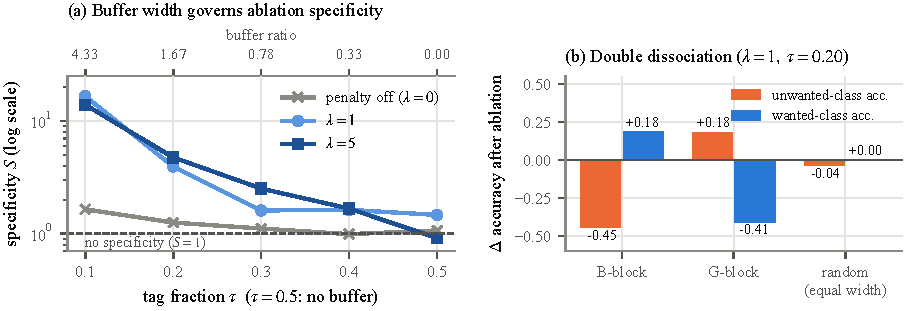
\includegraphics[width=\linewidth]{figures/fig_synthetic.pdf}
  \caption{\textbf{Synthetic testbed (\nSynthSeeds{} seeds).} (a) Ablation specificity $S$
  against tag fraction; the upper axis gives the buffer ratio. With the penalty off, $S\approx1$
  everywhere. With it on, $S$ is largest with a wide buffer and returns to chance when the buffer
  is removed. (b) At $\lambda=1,\tau=0.20$ each block selectively destroys its own class; a random
  block of equal width does neither.}
  \label{fig:synthetic}
\end{figure}

\begin{table}[!htbp]
  \centering\small
  \caption{\textbf{Specificity against buffer width} (synthetic, \nSynthSeeds{} seeds, mean $\pm$
  95\% CI). Removing the buffer returns the partition to chance.}
  \label{tab:spec}
  \begin{tabular}{@{}cc ccc ccc@{}}
\toprule
 & & \multicolumn{3}{c}{$\Delta$AUC, $\lambda=1$} & \multicolumn{3}{c}{Specificity $S$} \\
\cmidrule(lr){3-5}\cmidrule(l){6-8}
$\tau$ & Buffer ratio & B-block & Random block & & $\lambda=0$ & $\lambda=1$ & $\lambda=5$ \\
\midrule
0.10 & 4.33 & $-0.086\pm0.013$ & $-0.005\pm0.006$ & & 1.65 & \textbf{16.6} & 13.97 \\
0.20 & 1.67 & $-0.071\pm0.006$ & $-0.018\pm0.008$ & & 1.26 & \textbf{4.0} & 4.76 \\
0.30 & 0.78 & $-0.056\pm0.008$ & $-0.035\pm0.010$ & & 1.11 & \textbf{1.6} & 2.52 \\
0.40 & 0.33 & $-0.054\pm0.006$ & $-0.033\pm0.010$ & & 0.99 & \textbf{1.6} & 1.67 \\
0.50 & 0.00 & $-0.052\pm0.007$ & $-0.035\pm0.006$ & & 1.07 & \textbf{1.5} & 0.91 \\
\bottomrule
\end{tabular}
\end{table}

\Cref{fig:synthetic} and \cref{tab:spec} give the clearest view of what the partition does.
Without the penalty, specificity lies between \specOffMin{} and \specOffMax{} at every $\tau$:
reserving indices has no effect on its own. With the penalty ($\lambda=1$), specificity reaches
\specMax$\times$ at buffer ratio \specMaxBuf{} and falls to \specNoBufLamOne$\times$ as the buffer is
removed; at $\lambda=5$ the decline is strictly monotone and ends at \specNoBufLamFive, below chance. A smaller tagged
block with a wide buffer is both the most specific and the most effective configuration.

The ablations are cleanly dissociated (\cref{fig:synthetic}b, \cref{tab:dissociation}). Removing
$\Bset$ changes unwanted-class accuracy by $\dissBUnw$ and wanted-class accuracy by
$\dissBWan$; removing $\Gset$ mirrors this ($\dissGUnw$ and $\dissGWan$); a random block of equal
width changes them by $\dissRUnw$ and $\dissRWan$. Routing is \synthRouting{} with the
penalty against \synthRoutingOff{} without it, and $\Bset$ has \synthBAliveMin\% occupancy in
every penalised configuration, so the effect is not a silent-block artefact.

\begin{table}[!htbp]
  \centering\small
  \caption{\textbf{Double dissociation} (synthetic, $\lambda=1$, $\tau=0.20$, \nSynthSeeds{} seeds, mean $\pm$ 95\% CI).}
  \label{tab:dissociation}
  \begin{tabular}{@{}lccc@{}}
\toprule
Ablated block & $\Delta$acc.\ unwanted class & $\Delta$acc.\ wanted class & $\Delta$AUC \\
\midrule
B-block (unwanted side) & $-0.447\pm0.080$ & $+0.184\pm0.031$ & $-0.071\pm0.006$ \\
G-block (wanted side) & $+0.183\pm0.031$ & $-0.411\pm0.080$ & $-0.073\pm0.009$ \\
Random block, equal width & $-0.039\pm0.038$ & $+0.001\pm0.034$ & $-0.018\pm0.008$ \\
\bottomrule
\end{tabular}
\end{table}

\FloatBarrier
\subsection{Cross-group objectives, and why leakage misleads}
\label{sec:penform}

\begin{figure}[!htbp]
  \centering
  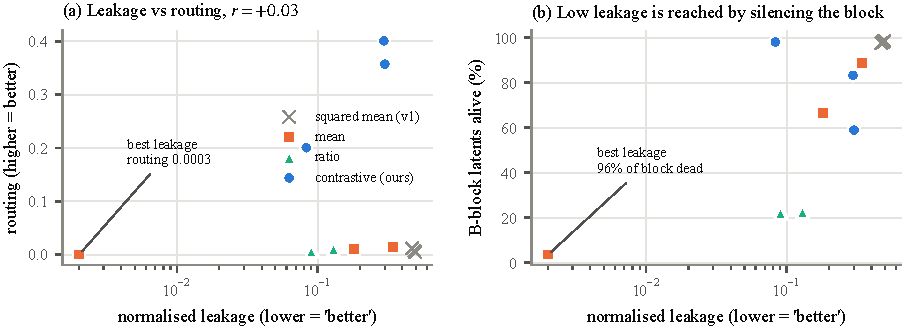
\includegraphics[width=\linewidth]{figures/fig_penform.pdf}
  \caption{\textbf{Penalty forms on GPT-2} (\penformConfigs{} configurations, $\tau=0.20$,
  \penformSeeds{} seeds each). (a) Leakage is uncorrelated with routing. (b) The configurations
  with the lowest leakage achieve it by silencing the unwanted block.}
  \label{fig:penform}
\end{figure}

\begin{table}[!htbp]
  \centering\small
  \caption{\textbf{Cross-group objectives} (GPT-2 L8 sentiment, $\tau=0.20$, mean of
  \penformSeeds{} seeds). Underlined: lowest leakage. Bold: highest routing.}
  \label{tab:penform}
  \begin{tabular}{@{}llccccc@{}}
\toprule
Objective & $\lambda$ & FVU $\downarrow$ & Leakage $\downarrow$ & Routing $\uparrow$ & B-block alive & Dead latents \\
\midrule
squared mean (v1) & 1 & 0.173 & 0.4936 & 0.005 & 99\% & 87 \\
 & 3 & 0.173 & 0.4861 & 0.008 & 98\% & 84 \\
 & 10 & 0.173 & 0.4705 & 0.012 & 97\% & 104 \\
\addlinespace[2pt]
mean & 1 & 0.175 & 0.3424 & 0.014 & 89\% & 308 \\
 & 3 & 0.179 & 0.1814 & 0.011 & 67\% & 834 \\
 & 10 & 0.188 & \underline{0.0020} & 0.000 & 4\% & 2380 \\
\addlinespace[2pt]
ratio & 1 & 0.188 & 0.0929 & 0.006 & 22\% & 1944 \\
 & 3 & 0.189 & 0.0900 & 0.006 & 22\% & 1994 \\
 & 10 & 0.190 & 0.1292 & 0.010 & 23\% & 1964 \\
\addlinespace[2pt]
\textbf{contrastive (ours)} & 1 & 0.250 & 0.3004 & 0.357 & 59\% & 1190 \\
 & 3 & 0.391 & 0.2955 & \textbf{0.401} & 83\% & 2533 \\
 & 10 & 1.026 & 0.0830 & 0.201 & 98\% & 3252 \\
\midrule
Vanilla TopK SAE & -- & 0.173 & -- & -- & -- & 82 \\
\bottomrule
\end{tabular}
\end{table}

The squared-mean penalty of the preliminary study does nothing at realistic sparsity. Raising
$\lambda$ from 0 to 30 moves normalised leakage only from \sqLeakLamZero{} to \sqLeakLamThirty{}
(chance is 0.5), and FVU varies by $\sqFVUspread$ across the whole sweep; at $\lambda=30$ the
penalty term is $\sqPenTermThirty$, \sqPenShare\% of the loss (\cref{tab:sqcalib}). Its routing
never exceeds \sqRoutMax.

Stronger suppression penalties lower leakage, but by the route \cref{prop:silent} predicts
(\cref{tab:penform}, \cref{fig:penform}). The lowest leakage of any configuration,
\bestLeakValue{} (\texttt{\bestLeakMode}, $\lambda=\bestLeakLambda$), comes with routing
\bestLeakRouting{} and \bestLeakDeadPct\% of the block dead. The contrastive objective has
\leakRatioBestVsRout$\times$ higher leakage (\bestRoutLeak) yet the highest routing (\bestRoutValue)
with \bestRoutAlivePct\% of the block alive. Across the \penformConfigs{} configurations, leakage and
routing are uncorrelated ($r=\leakRoutingCorr$). Leakage cannot be used to certify a partition.
Raw leakage is additionally not scale-invariant (\cref{tab:rescale}).

The contrastive objective costs reconstruction: at $\lambda=1$, FVU rises from \vanFVUpenform{} to
\contrastFVUlamOne{}, and at $\lambda=10$ to \contrastFVUlamTen, worse than predicting the mean. We
use $\lambda=1$ throughout; FVU for every run is reported in \cref{tab:quality}.

\FloatBarrier
\subsection{The reserved block localises the concept in language models}
\label{sec:block}

\begin{figure}[!htbp]
  \centering
  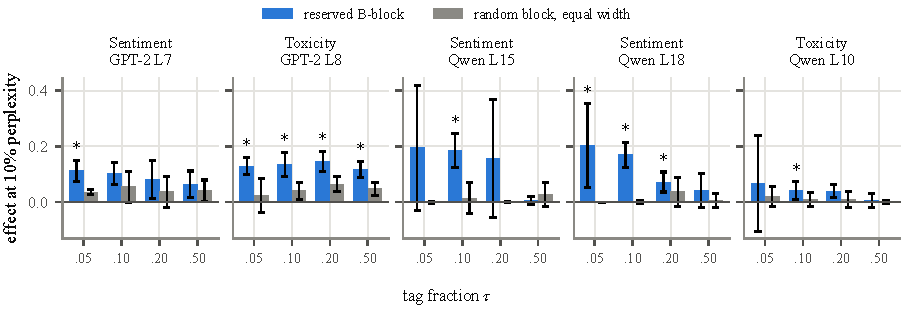
\includegraphics[width=\linewidth]{figures/fig_block.pdf}
  \caption{\textbf{Reserved block against a size-matched random block}, effect at a \budget\%
  perplexity budget (mean $\pm$ 95\% CI over seeds; $^{*}\,p<0.05$).}
  \label{fig:block}
\end{figure}

\begin{table}[!htbp]
  \centering\small
  \caption{\textbf{Reserved block minus size-matched random block}: mean difference in effect at a
  \budget\% budget\,/\,paired $p$-value. $^{\dagger}$Off-optimal layer (\cref{sec:layers}), reported
  for completeness and excluded from the counts in the text.}
  \label{tab:block}
  \begin{tabular}{@{}l cccc@{}}
\toprule
Run & $\tau=0.05$ & $\tau=0.10$ & $\tau=0.20$ & $\tau=0.50$ (no buffer) \\
\midrule
Sentiment, GPT-2, L7 & $+0.076$\,/\,0.010$^{*}$ & $+0.048$\,/\,0.229 & $+0.045$\,/\,0.181 & $+0.022$\,/\,0.352 \\
Toxicity, GPT-2, L8 & $+0.106$\,/\,0.015$^{*}$ & $+0.095$\,/\,0.002$^{*}$ & $+0.081$\,/\,0.018$^{*}$ & $+0.069$\,/\,0.013$^{*}$ \\
Sentiment, Qwen2.5-1.5B, L15 & $+0.196$\,/\,0.066 & $+0.171$\,/\,0.004$^{*}$ & $+0.156$\,/\,0.088 & $-0.023$\,/\,0.144 \\
Sentiment, Qwen2.5-1.5B, L18 & $+0.202$\,/\,0.029$^{*}$ & $+0.168$\,/\,0.003$^{*}$ & $+0.035$\,/\,0.044$^{*}$ & $+0.037$\,/\,0.111 \\
Toxicity, Qwen2.5-1.5B, L10 & $+0.046$\,/\,0.373 & $+0.032$\,/\,0.036$^{*}$ & $+0.031$\,/\,0.075 & $+0.005$\,/\,0.423 \\
\midrule
Toxicity, Qwen2.5-1.5B, L15$^{\dagger}$ & $+0.073$\,/\,0.149 & $+0.035$\,/\,0.095 & $+0.003$\,/\,0.476 & $+0.008$\,/\,0.367 \\
\bottomrule
\end{tabular}
\end{table}

Ablating $\Bset$ reduces the target behaviour more than ablating a random block of identical width
in \blockPositive{} of the \blockTotal{} run--$\tau$ cells (\cref{tab:block}, \cref{fig:block}; sign
test $p=\blockSignP$, treating cells as independent although they share evaluation prompts).
Individually, \blockSig{} cells reach $p<0.05$; with 3--5 seeds per cell, \blockSigHolm{} survives
Holm correction across all \blockTotal, so the evidence lies in the consistency of the direction
rather than in any single test. The effect concentrates where the buffer is wide: at $\tau=0.10$ it
is significant in \blockSigTauTen{} of \blockRuns{} runs, and at $\tau=0.50$ (no buffer) in
\blockSigTauFifty{} of \blockRuns. This reproduces, in two transformers and two concept axes, the
pattern of the synthetic testbed.

\FloatBarrier
\subsection{Against post-hoc selection and single-latent conditioning}
\label{sec:scale}

\begin{figure}[!htbp]
  \centering
  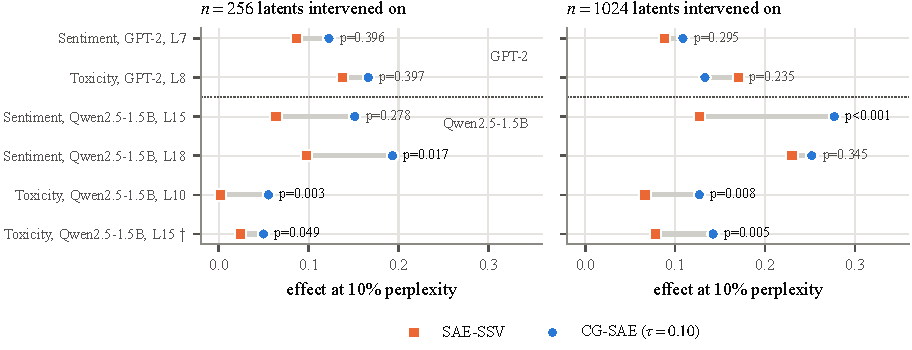
\includegraphics[width=\linewidth]{figures/fig_scale.pdf}
  \caption{\textbf{CG-SAE against the SAE-SSV-style control at matched intervention width.}
  Effect at a \budget\% budget; dotted line separates the two models. $^{\dagger}$Off-optimal layer.}
  \label{fig:scale}
\end{figure}

\begin{table}[!htbp]
  \centering\small
  \caption{\textbf{CG-SAE ($\tau=0.10$) against post-hoc and single-latent controls} at matched
  width $n$ (effect at a \budget\% budget; paired $p$ over seeds).}
  \label{tab:comparisons}
  \begin{tabular}{@{}l c c cc cc@{}}
\toprule
 & & & \multicolumn{2}{c}{SAE-SSV} & \multicolumn{2}{c}{Scar} \\
\cmidrule(lr){4-5}\cmidrule(l){6-7}
Run & $n$ & CG-SAE & effect & $p$ & effect & $p$ \\
\midrule
Sentiment, GPT-2, L7 & 256 & $+0.123$ & $+0.087$ & 0.396 & $+0.110$ & 0.806 \\
 & 1024 & $+0.109$ & $+0.088$ & 0.295 & $+0.118$ & 0.791 \\
\addlinespace[2pt]
Toxicity, GPT-2, L8 & 256 & $+0.166$ & $+0.138$ & 0.397 & $+0.122$ & 0.087 \\
 & 1024 & $+0.133$ & $+0.170$ & 0.235 & $+0.194$ & 0.091 \\
\midrule
Sentiment, Qwen2.5-1.5B, L15 & 256 & $+0.151$ & $+0.064$ & 0.278 & $+0.059$ & 0.336 \\
 & 1024 & $+0.277$ & $+0.127$ & $<$0.001$^{*}$ & $+0.147$ & 0.007$^{*}$ \\
\addlinespace[2pt]
Sentiment, Qwen2.5-1.5B, L18 & 256 & $+0.193$ & $+0.098$ & 0.017$^{*}$ & $+0.122$ & 0.081 \\
 & 1024 & $+0.252$ & $+0.230$ & 0.345 & $+0.250$ & 0.944 \\
\addlinespace[2pt]
Toxicity, Qwen2.5-1.5B, L10 & 256 & $+0.055$ & $+0.002$ & 0.003$^{*}$ & $+0.016$ & 0.084 \\
 & 1024 & $+0.127$ & $+0.066$ & 0.008$^{*}$ & $+0.075$ & 0.060 \\
\addlinespace[2pt]
Toxicity, Qwen2.5-1.5B, L15$^{\dagger}$ & 256 & $+0.050$ & $+0.024$ & 0.049$^{*}$ & $+0.031$ & 0.141 \\
 & 1024 & $+0.142$ & $+0.078$ & 0.005$^{*}$ & $+0.108$ & 0.117 \\
\bottomrule
\end{tabular}
\end{table}

Both arms here use the same post-hoc selection; they differ only in whether the dictionary was
trained with the partition. Holding intervention width fixed, CG-SAE does not outperform the
SAE-SSV-style control on GPT-2
(\vsSSVgptSig{} of \vsSSVgptTotal{} tests significant, $p=\vsSSVgptPmin$--$\vsSSVgptPmax$) but does
on Qwen2.5-1.5B, where the difference is positive in \vsSSVqwenPositive{} of \vsSSVqwenTotal{} tests
and significant in \vsSSVqwenSig{} (\vsSSVqwenSigHolm{} after Holm correction across the twelve;
\vsSSVqwenPrimSig{} of \vsSSVqwenPrimTotal{} excluding the off-optimal layer)
(\cref{tab:comparisons}, \cref{fig:scale}). The split is consistent across both concept axes,
but rests on two model sizes, so we read it as scale-\emph{associated} rather than
scale-\emph{dependent}. Against SCAR the comparison is weaker: \vsScarSig{} of \vsScarTotal{} tests
reach significance.

\FloatBarrier
\subsection{Against difference-in-means steering}
\label{sec:dim}

\begin{figure}[!htbp]
  \centering
  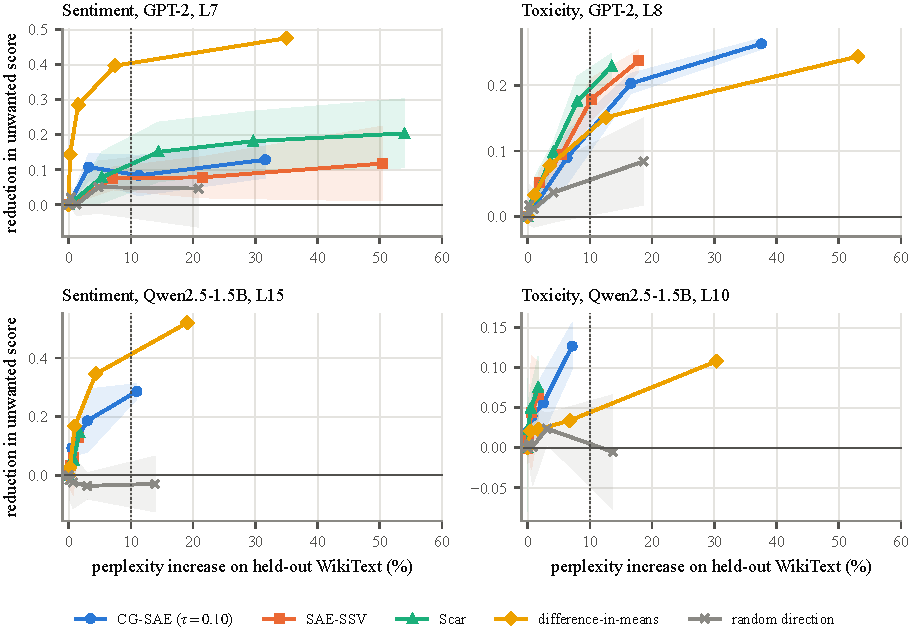
\includegraphics[width=\linewidth]{figures/fig_tradeoff.pdf}
  \caption{\textbf{Effect against fluency cost.} Mean over seeds with 95\% bands (none for the
  deterministic direction baselines). Dotted line: the \budget\% budget at which arms are compared.}
  \label{fig:tradeoff}
\end{figure}

\begin{table}[!htbp]
  \centering\small
  \caption{\textbf{Pre-specified SAE arms against difference-in-means} (effect at a \budget\% budget).
  Bold: significantly better than difference-in-means; italic: significantly worse
  ($^{*}\,p<0.05$). Arms were fixed in advance; no best-arm selection.}
  \label{tab:dim}
  \begin{tabular}{@{}l c cccc@{}}
\toprule
Run & Diff.-in-means & CG-SAE & SAE-SSV & Scar & CG-SAE block \\
\midrule
Sentiment, GPT-2, L7 & $+0.404$ & \textit{+0.109}$^{*}$ & \textit{+0.088}$^{*}$ & \textit{+0.118}$^{*}$ & \textit{+0.103}$^{*}$ \\
Toxicity, GPT-2, L8 & $+0.130$ & +0.133 & \textbf{+0.170}$^{*}$ & \textbf{+0.194}$^{*}$ & +0.135 \\
\midrule
Sentiment, Qwen2.5-1.5B, L15 & $+0.413$ & \textit{+0.277}$^{*}$ & \textit{+0.127}$^{*}$ & \textit{+0.147}$^{*}$ & \textit{+0.185}$^{*}$ \\
Sentiment, Qwen2.5-1.5B, L18 & $+0.374$ & \textit{+0.252}$^{*}$ & \textit{+0.230}$^{*}$ & \textit{+0.250}$^{*}$ & \textit{+0.169}$^{*}$ \\
Toxicity, Qwen2.5-1.5B, L10 & $+0.044$ & \textbf{+0.127}$^{*}$ & +0.066 & +0.075 & +0.042 \\
Toxicity, Qwen2.5-1.5B, L15$^{\dagger}$ & $+0.063$ & \textbf{+0.142}$^{*}$ & +0.078 & \textbf{+0.108}$^{*}$ & \textit{+0.045}$^{*}$ \\
\bottomrule
\end{tabular}
\end{table}

The ranking depends on the concept (\cref{fig:tradeoff}, \cref{tab:dim}). On sentiment,
difference-in-means beats every pre-specified SAE arm significantly in \dimSentSAEworse{} of
\dimSentTotal{} comparisons, at both scales. On toxicity no SAE arm is significantly worse, and
\dimToxSAEbetter{} of \dimToxTotal{} comparisons significantly favour the SAE arm: SAE-SSV and
SCAR on GPT-2 (SCAR $\scarGptTox$ against $\dimGptTox$, $p=\scarPGptTox$) and CG-SAE on Qwen ($\cgQwenTox$ against
$\dimQwenTox$, $p=\cgPQwenTox$). This agrees with the task-dependence reported by
\citet{xie2025comparative}. On sentiment the direction method's advantage is not an artefact of
degenerate text; repetition is essentially uncorrelated with measured effect
(\cref{app:degeneration}).

\FloatBarrier
\subsection{Where to intervene: decodability is not steerability}
\label{sec:layers}

\begin{figure}[!htbp]
  \centering
  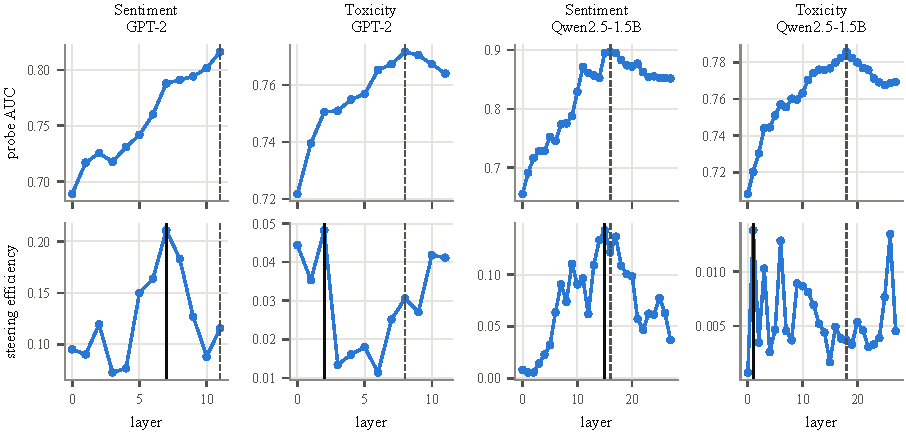
\includegraphics[width=\linewidth]{figures/fig_layers.pdf}
  \caption{\textbf{Layer scans.} Top: per-token linear-probe AUC. Bottom: steering efficiency
  (difference-in-means effect per unit perplexity cost, best of three strengths). Dashed: layer of
  maximal probe AUC; solid: layer of maximal steering efficiency.}
  \label{fig:layers}
\end{figure}

\begin{table}[!htbp]
  \centering\small
  \caption{\textbf{Probe optimum against steering optimum.} Last column: efficiency at the probe-AUC
  optimum as a fraction of the maximum.}
  \label{tab:layers}
  \begin{tabular}{@{}l c cc cc c@{}}
\toprule
 & & \multicolumn{2}{c}{Probe-AUC optimum} & \multicolumn{2}{c}{Steering optimum} & \\
\cmidrule(lr){3-4}\cmidrule(lr){5-6}
Scan & Layers & Layer & AUC & Layer & Effect / ppl & Eff.\ retained at probe optimum \\
\midrule
Sentiment, GPT-2 & 12 & 11 & 0.816 & 7 & $+0.278$\,/\,1.3\% & 55\% \\
Toxicity, GPT-2 & 12 & 8 & 0.772 & 2 & $+0.055$\,/\,1.1\% & 63\% \\
Sentiment, Qwen2.5-1.5B & 28 & 16 & 0.897 & 15 & $+0.148$\,/\,1.0\% & 85\% \\
Toxicity, Qwen2.5-1.5B & 28 & 18 & 0.786 & 1 & $+0.019$\,/\,1.4\% & 27\% \\
\bottomrule
\end{tabular}
\end{table}

For each layer we fit a per-token logistic probe and measured difference-in-means steering
efficiency (\cref{fig:layers}, \cref{tab:layers}). In all \layerScans{} scans the two optima
differ. On GPT-2 sentiment, probe AUC rises almost monotonically to the final layer
(L\layerGptProbe, \layerGptAUC) while efficiency peaks at L\layerGptSteer; choosing by probe AUC
forfeits \layerGptLoss\% of the achievable efficiency. Across scans, the probe optimum retains
\layerFracMin--\layerFracMax\% of the best efficiency. The practical cost of carrying a layer over
between tasks is sharp on Qwen: L15, optimal for sentiment, needs \qtoxLfifteenPPL\% perplexity to
reach an effect of $\qtoxLfifteenEff$ on toxicity, which L10 reaches at \qtoxLtenPPL\%
($\qtoxLtenEff$). The toxicity scans are noisier than the sentiment scans because the steering signal
is weak, and their efficiency optima (L2, L1) should be read with that in mind; the disagreement
between the two criteria does not depend on them.

A plausible reading is that late layers are highly decodable because the residual stream is
already committed to the next token, while an edit there has little downstream computation
through which to act. This is consistent with the view that probe accuracy measures presence,
not use~\citep{hewitt2019control,belinkov2022probing}, and bears on methods that choose
intervention sites by probe accuracy~\citep{li2023iti}.

% ===========================================================================
\FloatBarrier
\section{Discussion}
\label{sec:discussion}

\paragraph{Why the buffer matters.}
Some features are genuinely shared between the two classes. With no buffer they must be assigned
to one side, where the penalty either pushes them out (costing reconstruction) or they remain and
contaminate that side. The buffer gives them a home, so the tagged blocks can specialise. The
synthetic testbed shows this directly: specificity is a monotone function of buffer width, and is
at chance without a buffer even when the penalty is on.

\paragraph{Localisation without a universal steering advantage.}
The reserved block demonstrably contains the concept, yet removing it steers no better than
post-hoc selection on a vanilla SAE on GPT-2, and worse than a difference-in-means direction
on sentiment. These are
different properties. Localisation asks whether a region is specific; steering efficiency asks
how much behaviour change is bought per unit of fluency. A block can be specific without being the
most efficient lever. What the block offers that post-hoc selection does not is an intervention
fixed at training time, which is auditable and requires no labelled data at deployment.

\paragraph{Implications for evaluation.}
Two practices common in this area can mislead: certifying a partition by leakage, and choosing a
layer by probe accuracy. Both measure something real, but not the property they are used to
certify. We recommend reporting routing and occupancy alongside any leakage figure, evaluating
interventions at a matched fluency budget, and selecting intervention sites by intervention.

% ===========================================================================
\FloatBarrier
\section{Limitations}
\label{sec:limits}
\begin{itemize}
  \item \textbf{Two model sizes.} The larger-scale advantage over post-hoc selection is observed on
        one model of each size; more sizes are needed to call it a scaling trend.
  \item \textbf{Few seeds.} Three to five seeds per cell leave single comparisons underpowered;
        our strongest claims rest on consistency across cells, not on individual $p$-values.
  \item \textbf{Reconstruction cost.} The contrastive objective raises FVU relative to a vanilla SAE,
        and the Qwen dictionaries contain many dead latents because we used no auxiliary
        dead-latent loss. FVU is also not comparable across models: Qwen's residual stream has
        a few very high-variance dimensions, which lowers FVU without implying better fine-grained
        reconstruction.
  \item \textbf{Token-level splits.} SAE train, validation and test tokens are split at the token level,
        so metrics computed on SAE codes (FVU, routing, selectivity) may be optimistic. Steering
        and perplexity are evaluated on held-out documents and are not affected.
  \item \textbf{Automatic judges.} Effects are measured by classifiers; we check for degeneration
        with distinct-2, but ran no human evaluation. For Qwen distinct-2 is at ceiling and is
        uninformative.
  \item \textbf{Scope.} Two binary concept axes, inference-time intervention only; multi-concept
        partitions and weight editing are untested.
\end{itemize}

% ===========================================================================
\section{Conclusion}
\label{sec:conclusion}
Reserving a labelled block of SAE latent capacity for an unwanted behaviour, separated from the
rest by an unpenalised buffer, produces a region that demonstrably contains the concept and can be
removed by address rather than by search. The buffer, not the partition alone, is what makes the
region specific. Making this work required an objective that suppression-style penalties cannot
supply, and evaluating it required measures that leakage cannot supply. Whether the reserved block
is the best steering lever depends on scale and task. The full pipeline, including the scripts
that generate every number, table and figure in this paper, will be released with the final
version.

\paragraph{Reproducibility.}
All experiments ran on Kaggle (NVIDIA P100, 16\,GB). Source code, run configurations, raw result
tables and the asset-generation script are in the project repository under \texttt{cgsae/}; every
number in this paper is produced by \texttt{paper/make\_paper\_assets.py} from those tables.

\paragraph{Ethics.}
Toxicity experiments use RealToxicityPrompts; we do not reproduce model generations for that axis.
The techniques studied here are aimed at reducing unwanted behaviour, and removal by address could
in principle be reversed to amplify it.

{\small
\bibliographystyle{plainnat}
\bibliography{references}
}

% ===========================================================================
\clearpage
\appendix
\section{Audit of the preliminary implementation}
\label{app:audit}

This paper supersedes our earlier report on CG-SAE. Before running new experiments we audited that
implementation. \Cref{tab:audit} lists what we found and what replaced it. The first row is the
most consequential: the reported steering and perplexity results selected latents over the whole
latent space, so they measured post-hoc selection rather than the partition.

\begin{table}[!htbp]
  \centering\small
  \caption{\textbf{Issues in the preliminary implementation and their resolution.}}
  \label{tab:audit}
  \begin{tabular}{@{}p{0.34\linewidth}p{0.29\linewidth}p{0.29\linewidth}@{}}
  \toprule
  Issue in preliminary study & Consequence & Resolution in this work \\
  \midrule
  Steering latents ranked over all 768 latents, not the B-block
    & Headline steering result never used the partition
    & Block arm ablates $\Bset$ by address; size-matched random-block null \\
  Unsteered text sampled ($T{=}0.7$, top-$p$ 0.9), steered text greedy
    & Before/after differences confounded with decoder
    & Greedy decoding for every arm \\
  SAE trained on mean-pooled reviews, applied per token
    & Train/test distribution mismatch
    & Per-token activations throughout \\
  $d_{\mathrm{latent}}=d_{\mathrm{in}}=768$, $L_0\approx394$
    & Dense, not sparse, autoencoder
    & TopK, $m=8d$, $L_0=32$ exactly \\
  No vanilla-SAE or baseline arm
    & Central claim untestable
    & SAE-SSV and SCAR controls, direction baselines, three nulls \\
  Pruning measured by per-class accuracy at a fixed threshold
    & A shifted decision boundary reads as asymmetry
    & Threshold-free AUC; random- and G-block controls \\
  $n=100$ test set, single seed, configuration chosen by the reported metric
    & Effects within noise
    & 3--20 seeds, paired tests, Holm correction \\
  Perplexity on 10 prompts, last 5 positions edited, raw-decode replacement
    & Cost measured where it is smallest; includes SAE error
    & Held-out WikiText, all positions, delta-form edit \\
  Leakage as mean off-group activation
    & Scale-gameable; silent blocks score perfectly
    & Routing and occupancy reported alongside \\
  Squared-mean cross-group penalty
    & Inert under real sparsity; admits silent minimiser
    & Contrastive routing objective \\
  \bottomrule
  \end{tabular}
\end{table}

\FloatBarrier
\section{Hyperparameters, runs and compute}
\label{app:hparams}

\begin{table}[!htbp]
  \centering\small
  \caption{\textbf{Hyperparameters.}}
  \label{tab:hparams}
  \begin{tabular}{@{}ll@{}}
  \toprule
  Setting & Value \\
  \midrule
  SAE width $m$ & $8d$ (6{,}144 for GPT-2; 12{,}288 for Qwen) \\
  Sparsity & TopK, $k=32$ \\
  Optimiser & Adam~\citep{kingma2015adam}, lr $3\times10^{-4}$, batch 4{,}096, 30 epochs \\
  Decoder & tied initialisation, unit-norm rows re-normalised each step \\
  Cross-group objective & $P_{\mathrm{con}}$, $\lambda=1$ \\
  Tag fractions $\tau$ & $\{0.05,0.10,0.20,0.50\}$ \\
  SCAR control & BCE on pre-activation of latent 0, weight 1 \\
  Selection gate & firing rate $\ge10^{-3}$ on validation tokens (40k subsample) \\
  Intervention width $n$ & $\{64,256,1024\}$; block $=\ntag$ \\
  SAE strengths $\alpha$ & $\{0,0.25,0.5,0.75,1\}$ \\
  Direction strengths & $\{0,0.5,1,2,4,8\}$, scale $s=\E\|\x\|\sigma/10$ \\
  Generation & greedy, 32 new tokens, prompts truncated to 128 tokens \\
  Perplexity corpus & 150 WikiText-103 test paragraphs ($\ge40$ words), 128 tokens \\
  Budget & \budget\% perplexity increase \\
  Layer scans & 120k tokens, 96 prompts, strengths $\{1,2,4\}$, difference-in-means \\
  \bottomrule
  \end{tabular}
\end{table}

\begin{table}[!htbp]
  \centering\small
  \caption{\textbf{Run inventory}, read from the saved run configurations. $^{\dagger}$Off-optimal layer.}
  \label{tab:inventory}
  \begin{tabular}{@{}l l c c c c c@{}}
\toprule
Run & Model & Layer & Seeds & Tokens & $d_{\text{latent}}$ & Unsteered PPL \\
\midrule
R1 & GPT-2 & 7 & 5 & 600{,}000 & 6{,}144 & 52.13 \\
R2 & GPT-2 & 8 & 5 & 172{,}330 & 6{,}144 & 52.13 \\
R3 & Qwen2.5-1.5B & 15 & 3 & 300{,}000 & 12{,}288 & 16.89 \\
R4 & Qwen2.5-1.5B & 18 & 3 & 300{,}000 & 12{,}288 & 16.89 \\
R5 & Qwen2.5-1.5B & 10 & 3 & 169{,}439 & 12{,}288 & 16.89 \\
R6$^{\dagger}$ & Qwen2.5-1.5B & 15 & 3 & 169{,}439 & 12{,}288 & 16.89 \\
\bottomrule
\end{tabular}
\end{table}

\paragraph{Compute.} Every run used a single NVIDIA P100 (16\,GB) on Kaggle; the Qwen runs were
the most expensive because generation dominates the cost of the strength sweeps.

\FloatBarrier
\section{Extended results}
\label{app:extended}

\begin{table}[!htbp]
  \centering\small
  \caption{\textbf{SAE quality per run} (mean $\pm$ s.d.\ over seeds). Routing and occupancy are
  defined only for CG-SAE. Dead latents: latents that never fire on a 40k-token validation subsample.}
  \label{tab:quality}
  \begin{tabular}{@{}ll ccccc@{}}
\toprule
Run & SAE & FVU & L$_0$ & Routing & B-block alive & Dead latents \\
\midrule
Sent., GPT-2 L7 & Vanilla & 0.162$\pm$0.000 & 32 & -- & -- & 92 \\
 & Scar & 0.163$\pm$0.000 & 32 & -- & -- & 103 \\
 & CG-SAE $\tau=0.05$ & 0.215$\pm$0.001 & 32 & 0.326 & 70\% & 653 \\
 & CG-SAE $\tau=0.10$ & 0.221$\pm$0.001 & 32 & 0.329 & 60\% & 850 \\
 & CG-SAE $\tau=0.20$ & 0.236$\pm$0.001 & 32 & 0.331 & 63\% & 1185 \\
 & CG-SAE $\tau=0.50$ & 0.264$\pm$0.000 & 32 & 0.341 & 79\% & 1409 \\
\addlinespace[3pt]
Toxi., GPT-2 L8 & Vanilla & 0.244$\pm$0.000 & 32 & -- & -- & 77 \\
 & Scar & 0.245$\pm$0.001 & 32 & -- & -- & 80 \\
 & CG-SAE $\tau=0.05$ & 0.322$\pm$0.001 & 32 & 0.332 & 51\% & 498 \\
 & CG-SAE $\tau=0.10$ & 0.333$\pm$0.000 & 32 & 0.336 & 57\% & 702 \\
 & CG-SAE $\tau=0.20$ & 0.335$\pm$0.000 & 32 & 0.353 & 69\% & 940 \\
 & CG-SAE $\tau=0.50$ & 0.336$\pm$0.000 & 32 & 0.364 & 82\% & 1131 \\
\addlinespace[3pt]
Sent., Qwen L15 & Vanilla & 0.045$\pm$0.002 & 32 & -- & -- & 1826 \\
 & Scar & 0.046$\pm$0.002 & 32 & -- & -- & 1925 \\
 & CG-SAE $\tau=0.05$ & 0.061$\pm$0.002 & 32 & 0.500 & 28\% & 4027 \\
 & CG-SAE $\tau=0.10$ & 0.065$\pm$0.001 & 32 & 0.518 & 34\% & 4387 \\
 & CG-SAE $\tau=0.20$ & 0.070$\pm$0.002 & 32 & 0.545 & 53\% & 6428 \\
 & CG-SAE $\tau=0.50$ & 0.070$\pm$0.003 & 32 & 0.551 & 48\% & 6301 \\
\addlinespace[3pt]
Sent., Qwen L18 & Vanilla & 0.094$\pm$0.014 & 32 & -- & -- & 1846 \\
 & Scar & 0.095$\pm$0.014 & 32 & -- & -- & 1945 \\
 & CG-SAE $\tau=0.05$ & 0.127$\pm$0.015 & 32 & 0.501 & 30\% & 3802 \\
 & CG-SAE $\tau=0.10$ & 0.135$\pm$0.015 & 32 & 0.512 & 39\% & 4185 \\
 & CG-SAE $\tau=0.20$ & 0.142$\pm$0.014 & 32 & 0.537 & 56\% & 6182 \\
 & CG-SAE $\tau=0.50$ & 0.140$\pm$0.014 & 32 & 0.543 & 48\% & 6130 \\
\addlinespace[3pt]
Toxi., Qwen L10 & Vanilla & 0.018$\pm$0.000 & 32 & -- & -- & 1280 \\
 & Scar & 0.018$\pm$0.000 & 32 & -- & -- & 1285 \\
 & CG-SAE $\tau=0.05$ & 0.031$\pm$0.000 & 32 & 0.415 & 99\% & 2815 \\
 & CG-SAE $\tau=0.10$ & 0.030$\pm$0.000 & 32 & 0.413 & 99\% & 3963 \\
 & CG-SAE $\tau=0.20$ & 0.028$\pm$0.000 & 32 & 0.402 & 98\% & 4833 \\
 & CG-SAE $\tau=0.50$ & 0.025$\pm$0.000 & 32 & 0.389 & 95\% & 585 \\
\addlinespace[3pt]
Toxi., Qwen L15 & Vanilla & 0.021$\pm$0.000 & 32 & -- & -- & 1692 \\
 & Scar & 0.021$\pm$0.000 & 32 & -- & -- & 1696 \\
 & CG-SAE $\tau=0.05$ & 0.036$\pm$0.000 & 32 & 0.441 & 99\% & 3135 \\
 & CG-SAE $\tau=0.10$ & 0.034$\pm$0.000 & 32 & 0.441 & 99\% & 4395 \\
 & CG-SAE $\tau=0.20$ & 0.032$\pm$0.000 & 32 & 0.433 & 98\% & 5138 \\
 & CG-SAE $\tau=0.50$ & 0.029$\pm$0.000 & 32 & 0.421 & 94\% & 744 \\
\bottomrule
\end{tabular}
\end{table}

\begin{table}[!htbp]
  \centering\small
  \caption{\textbf{Calibration of the squared-mean penalty} (GPT-2 L8 sentiment, $\tau=0.20$, one seed).}
  \label{tab:sqcalib}
  \begin{tabular}{@{}cccc@{}}
\toprule
$\lambda$ & Normalised leakage & Raw leakage & FVU \\
\midrule
0 & 0.4945 & 0.0136 & 0.17392 \\
1 & 0.4901 & 0.0121 & 0.17388 \\
3 & 0.4832 & 0.0107 & 0.17384 \\
10 & 0.4654 & 0.0078 & 0.17389 \\
30 & 0.4353 & 0.0054 & 0.17397 \\
\bottomrule
\end{tabular}
\end{table}

\begin{table}[!htbp]
  \centering\small
  \caption{\textbf{Raw leakage is not scale-invariant.} A rescaling that leaves separation unchanged
  divides raw leakage by the scale factor; normalised leakage is unaffected.}
  \label{tab:rescale}
  \begin{tabular}{@{}ccc@{}}
\toprule
Scale $c$ ($\mathbf z\mapsto c\,\mathbf z$) & Raw leakage & Normalised leakage \\
\midrule
1 & 0.12310 & 0.20126 \\
0.1 & 0.01231 & 0.20126 \\
0.01 & 0.00123 & 0.20126 \\
\bottomrule
\end{tabular}
\end{table}

\FloatBarrier
\section{Degeneration check}
\label{app:degeneration}

A judge score cannot tell a genuine sentiment shift from text that has degenerated into
repetition~\citep{holtzman2020degeneration}. We compute distinct-2, the fraction of unique bigrams,
for every saved generation and correlate it with measured effect across all operating points of a
run (\cref{tab:degen}). The strongest correlation is $\degenCorrMax$. On GPT-2 the difference-in-means
direction at $\alpha=4$ produces text no more repetitive than the unsteered model; it degenerates
only at $\alpha=8$, far beyond the \budget\% budget used for comparison. Qwen's completions contain
no repeated bigrams at any operating point, so distinct-2 is at ceiling and uninformative there.

\begin{table}[!htbp]
  \centering\small
  \caption{\textbf{Repetition and measured effect} (sentiment runs).}
  \label{tab:degen}
  \begin{tabular}{@{}l ccc@{}}
\toprule
Run & Unsteered distinct-2 & corr(effect, distinct-2) & Diff.-in-means distinct-2 at $\alpha{=}4$ \\
\midrule
Sentiment, GPT-2, L7 & 0.661 & $-0.11$ & 0.718 \\
Sentiment, Qwen2.5-1.5B, L15 & 1.000 & $-0.28$ & 1.000 \\
Sentiment, Qwen2.5-1.5B, L18 & 1.000 & $-0.26$ & 1.000 \\
\bottomrule
\end{tabular}
\end{table}

\FloatBarrier
\section{Qualitative examples}
\label{app:qualitative}

\Cref{tab:qual} shows GPT-2 continuations of two held-out negative-review openings (first seed).
At full strength every family of intervention can degenerate: the CG-SAE block and SAE-SSV
($n=1024$) at $\alpha=1$ fall into repetition, as does difference-in-means at $\alpha=8$. This
is why arms are compared at a fixed fluency budget rather than at maximal effect. Note also
that unsteered GPT-2 is itself repetitive, which is why its distinct-2 baseline is low.

\begin{table}[!htbp]
  \centering\small
  \caption{\textbf{GPT-2 L7 continuations} under selected interventions.}
  \label{tab:qual}
  \begin{tabular}{@{}p{0.26\linewidth}p{0.68\linewidth}@{}}
\toprule
\multicolumn{2}{@{}l}{\textbf{Prompt:} \emph{Specks of white and various shapes, a beautiful nude, random}} \\
\midrule
Unsteered & shapes, and a few other things.  I'm not sure if I'm going to be able to do this, but I'm going to be able \\
CG-SAE block, $\alpha=1$ & , and a little bit of a white, and a little bit of a black, and a little bit of a black, and a little bit of a white \\
SAE-SSV, $n=1024$, $\alpha=1$ & , and a very beautiful, beautiful, beautiful, beautiful, beautiful, beautiful, beautiful, beautiful, beautiful, beautiful, beautiful, beautiful, beautiful, beautiful, \\
Diff.-in-means, $\alpha=2$ & , and a very special one.  The first time I saw the statue was in the summer of 2013. It was a beautiful, beautiful statue of a \\
Diff.-in-means, $\alpha=8$ & and a young and unique family, the family of the family of the family of the family of the family of the family of the family of the family of the \\
\midrule
\multicolumn{2}{@{}l}{\textbf{Prompt:} \emph{This is one of the worst films I've seen for}} \\
\midrule
Unsteered & a while. It's a very dark, dark, dark movie. It's a very dark movie. It's a very dark movie. It's a very \\
CG-SAE block, $\alpha=1$ & me, and I'm not sure what to say to the people who have been asking for it. I'm not sure what to say to the people who have \\
SAE-SSV, $n=1024$, $\alpha=1$ & a while now. It's a very dark film, and it's very dark. It's a very dark film. It's a very dark film. It \\
Diff.-in-means, $\alpha=2$ & a while. It's a very dark and dark story, and it's very dark and dark. It's a very dark story, and it's very dark \\
Diff.-in-means, $\alpha=8$ & me. It is a story of the journey of the family, the journey of the family, the journey of the family, the journey of the family, the \\
\bottomrule
\end{tabular}
\end{table}

\FloatBarrier
\section{Implementation}
\label{app:code}

The core components, lightly abridged from \texttt{cgsae/src/}.

\medskip\noindent\textbf{TopK encoding (all SAE arms).}\par\nobreak\smallskip
\begin{lstlisting}[style=py]
def encode(self, x):
    pre = F.relu((x - self.b_pre) @ self.W_enc + self.b_enc)
    vals, idx = torch.topk(pre, self.k, dim=-1)          # exactly k active latents
    return torch.zeros_like(pre).scatter_(-1, idx, vals)
\end{lstlisting}

\medskip\noindent\textbf{Contrastive routing objective.}\par\nobreak\smallskip
\begin{lstlisting}[style=py]
def aux_loss(self, z, labels, pre):                         # labels: 1 wanted, 0 unwanted
    pos, neg = labels == 1, labels == 0
    total   = z.sum(-1) + EPS                               # total mass, buffer included
    g_share = z[:, self.g_idx].sum(-1) / total
    b_share = z[:, self.b_idx].sum(-1) / total
    pen = -0.5 * ((b_share[neg].mean() - b_share[pos].mean())
                  + (g_share[pos].mean() - g_share[neg].mean()))
    return self.lambda_cg * pen                             # silence scores 0, routing -1
\end{lstlisting}

\medskip\noindent\textbf{Delta-form intervention.}\par\nobreak\smallskip
\begin{lstlisting}[style=py]
def make_sae_edit(sae, latent_idx, alpha, mu, sigma):
    idx = torch.as_tensor(latent_idx, device=mu.device)
    def edit(h):
        x  = (h.float() - mu) / sigma
        z  = sae.encode(x)
        z2 = z.clone(); z2[..., idx] *= (1.0 - alpha)
        # only the change is added: reconstruction error never enters the stream
        return (h.float() + (sae.decode(z2) - sae.decode(z)) * sigma).to(h.dtype)
    return None if alpha == 0.0 else edit
\end{lstlisting}

\medskip\noindent\textbf{Effect at a matched budget.}\par\nobreak\smallskip
\begin{lstlisting}[style=py]
def effect_at_budget(sweep, budget):
    s = sweep.sort_values("ppl_pct")
    x, y = s["ppl_pct"].values, s["effect"].values
    if budget >= x.max():
        return y[np.argmax(x)]
    return np.interp(budget, x, np.maximum.accumulate(y))   # upper envelope
\end{lstlisting}

\end{document}
